\subsection{Taylor Series and Calculation of Fuctions}

\frame{
For example
\begin{itemize}
\item the derivative 
\begin{equation*}
f'(x) = lim_{h \to 0} \frac{f(x+h) - f(x)}{h}
\end{equation*}
 is the limit of the difference quotient where both the numerator and the denominator go to zero.
\item A Taylor series illustrates another type of limit process. In this case an infinite number of terms is added together by taking the limit of certain partial sums. 
\item An important application is their use to represent the elementary functions: $\sin(x)$, $\cos(x)$, $e^x$, $In(x)$, etc. 
\end{itemize}
}

\frame{
\begin{itemize}
\item Table 3.1 gives several of the common Taylor series expansions. 
\item The partial sums can be accumulated until an approximation to the function is obtained that has the accuracy specified. 
\item Series solutions are used in the areas of engineering and physics. 
\end{itemize}
\begin{figure}
\begin{center}
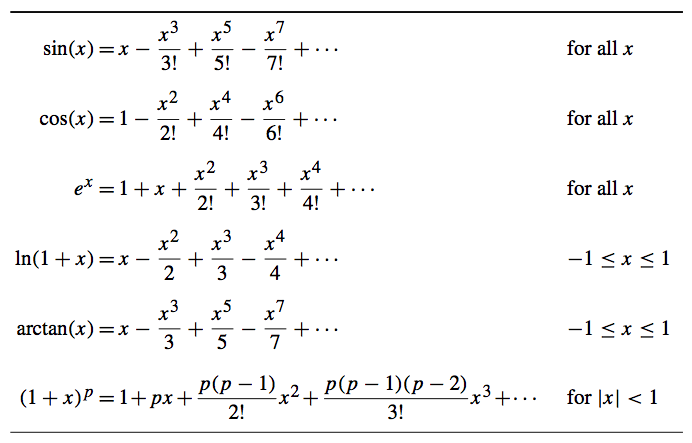
\includegraphics[width=80mm]{chap-3/tab_4-1.png}
\end{center}
\end{figure}
}

\frame{
\begin{itemize}
\item We want to learn how a finite sum can be used to obtain a good approximation to an infinite sum. 
\item For illustration we shall use the exponential series in the above table  to compute the number $e = e^1$, which is the base of the natural logarithm and exponential functions. 
\item Here we choose $x = 1$ and use the series 
\begin{equation*}
e^1 = 1 + \frac{1}{1!} + \frac{1^2}{2!} + \frac{1^3}{3!} + \frac{1^4}{4!} + \cdots + \frac{1^k}{k!} + \cdots 
\end{equation*}
\end{itemize}
}

\frame{
The definition for the sum of an infinite series requires that the partial sums $S_N$ tend to a limit. 
The values of these sums are given in the following table. 
\begin{figure}
\begin{center}
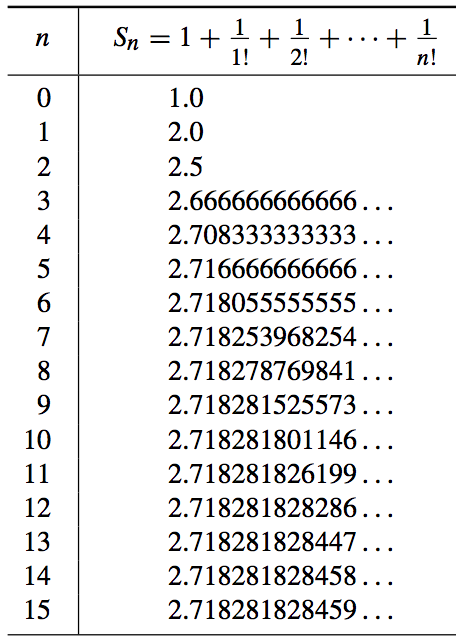
\includegraphics[width=50mm]{chap-3/tab_4-2.png}
\end{center}
\end{figure}
}

\frame{
\begin{itemize}
\item A natural way to think about the power series representation of a function is to view the expansion as the limiting case of polynomials of increasing degree. 
\item If enough terms are added, then an accurate approximation will be obtained. 
\item This needs to be made precise. 
\end{itemize}
\begin{block}{What degree should be chosen for the polynomial, and how do we calculate the coefficients for the powers of x in the polynomial? }
Theorem 3.1 answers these questions.
\end{block}
}

\frame{
\begin{block}{Theorem 3.1 (Taylor Polynomial Approximation).}
Assume that $f \in C^{N+l} [a, b]$ and $x_0 \in [a, b]$ is a fixed value. 
If $x \in [a, b]$, then 
\begin{equation*}
f(x) = P_N(x) + E_N(x)
\end{equation*}
where $P_N(x)$ is a polynomial that can be used to approximate $f(x)$ : 
\begin{equation*}
f(x) \approx P_N(x) = \sum_{k=0}^N \frac{f^{(k)}(x_0)}{k!} \left( x-x_0 \right)^k
\end{equation*}
The error term $E_N (x)$ has the form 
\begin{equation*}
E_N(x) = \frac{f^{(N+1)}(c)}{\left( N+1 \right)!} \left( x-x_0 \right)^{N+1}
\end{equation*}
for some value $c = c(x)$ that lies between $x$ and $x_0$
\end{block}
}

\frame{
\begin{itemize}
\item Relation (3.2) indicates how the coefficients of the Taylor polynomial are calculated. 
\item Although the error term (3.3) involves a similar expression, notice that $f^{(N+1)}(c)$ is to be evaluated at an undetermined number $c$ that depends on the value of $x$. 
\item For this reason we do not try to evaluate $E_N(x)$ : it is used to determine a bound for the accuracy of the approximation. 
\end{itemize}
}

\frame{
\frametitle{Example 3.1.}
Show why 15 terms are all that are needed to obtain the 13-digit approximation $e = 2.718281828459$ in Table 3.2. 
\begin{itemize}
\item Expand $f(x) = e^x$ in a Taylor polynomial of degree $15$ using the fixed value $x_0 = 0$ and involving the powers $(x - 0)^k = x^k$. 
\item The derivatives required are $f`(x) = f``(x) = \cdots = f^{(16)} = e^x$. 
\item The first $15$ derivatives are used to calculate the coefficients $a_k = e^0 / k!$ and are used to write
\begin{equation*}
P_{15}(x) = 1 + x + \frac{x^2}{2!} + \frac{x^3}{3!} + \cdots + \frac{x^{15}}{15!}
\end{equation*}
\end{itemize}
Setting $x = 1$ in (3.4) gives the partial sum $S_{15} = P_{15}(1)$. 
The remainder term is needed to show the accuracy of the approximation: 
\begin{equation*}
E_{15}(x) = \frac{f^{(16)}(c)x^{16}}{16!}
\end{equation*}
}

\frame{
\begin{itemize}
\item Since we chose $x_0 = 0$ and $x = 1$, the value $c$ lies between them (i.e., $0 < c < 1$), which implies that $e^c < e^1$. 
\item Notice that the partial sums in Table 3.2 are bounded above by $3$. 
\item Combining these two inequalities yields $e^c < 3$, which is used in the following calculation
\begin{equation*}
\left| E_{15}(1) \right| = \frac{\left| f^{(16)}(c) \right|}{16!} = \frac{e^c}{16!} < \frac{3}{16!} < 1.433844 \times 10^{-13}
\end{equation*}
\end{itemize}
\begin{block}{}
Therefore, all the digits in the approximation $e \approx 2.718281828459$ are correct, because the actual error (whatever it is) must be less than $2$ in the thirteenth decimal place. 
\end{block}
}

\frame{
\begin{itemize}
\item Instead of giving a rigorous proof of Theorem 3.1, we shall discuss some of the features of the approximation; the reader can look in any standard reference text on calculus for more details. 
\item For illustration, we again use the function $f(x) = e^x$ and the value $x_0 = 0$. 
\item From elementary calculus we know that the slope of the curve $y = e^x$ at the point $(x, e^x)$ is $f'(x) = e^x$. 
\item Hence the slope at the point $(0,1)$ is $1'(0) = 1$.
\item Therefore, the tangent line to the curve at the point $(0,1)$ is $y = 1 + x$. 
\item This is the same formula that would be obtained if we used $N = 1$ in Theorem 3.1;  that is, $P_1 (x) = f(0) + f'(0)x/1! = 1 + x$. 
\end{itemize}
}

\frame{
Therefore, $P_1(x)$ is the equation of the tangent line to the curve. 
The graphs are shown in Figure 3.3.
\begin{figure}
\begin{center}
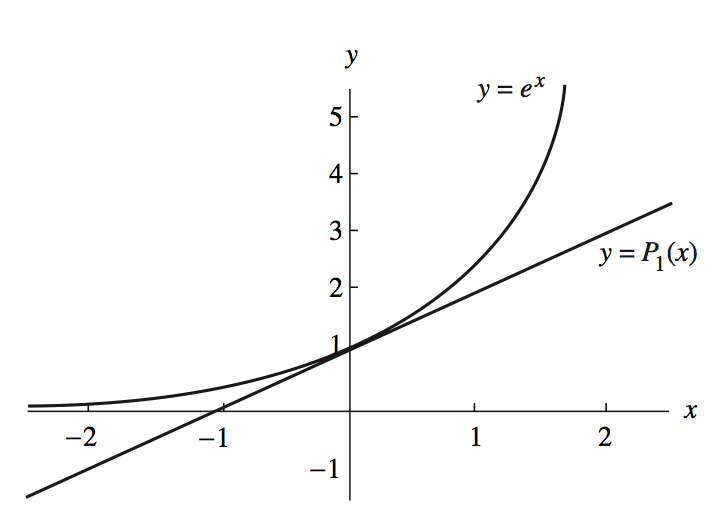
\includegraphics[width=60mm]{chap-3/fig_4-3.png}
\end{center}
\end{figure}
}

\frame{
\begin{itemize}
\item Observe that the approximation $e^x \approx 1 + x$ is good near the center $x_0 = 0$ and that the distance between the curves grows as $x$ moves away from $0$. 
\item Notice that the slopes of the curves agree at $(0,1)$. 
\item In calculus we learned that the second derivative indicates whether a curve is concave up or down. 
\item The study of curvature1 shows that if two curves $y = f(x)$ and $y = g(x)$ have the property that $f(x_0) = g(x_0)$, $f'(x_0) = g'(x_0)$, and $f"(x_0) = g"(x_0)$ then they have the same curvature at $x_0$. 
\item This property would be desirable for a polynomial function that approximates $f(x)$. 
\end{itemize}
\begin{block}{}
Corollary 3.1 shows that the Taylor polynomial has this property for $N \ge 2$. 
\end{block}
}

\frame{
\begin{block}{Corollary 3.1. }
 If $P_N(x)$ is the Taylor polynomial of degree $N$ given in Theorem 3.1, then 
\begin{equation*}
P_N^{(k)} (x_0) = f^{(k)}(x_0) \ \ \ \ \ \ for \ \  k = 0, 1, \ldots N 
\end{equation*}
\end{block}
Proof : \\
Set $x = x_0$ in equations (3.2) and (3.3), and the result is $P_N(x_0) = f(x_0)$. 
Thus statement (3,6) is true for $k = 0$. 
Now differentiate the right-hand side of (3.2) and get 
\begin{equation*}
P`_N(x) = \sum_{k = 1}^{N} \frac{f^{(k)}(x_0)}{(k-1)!} (x - x_0)^{k-1} = \sum_{k = 0}^{N-1} \frac{f^{(k+1)}(x_0)}{k!} (x - x_0)^{k}
\end{equation*}
Set $x = x_0$ in (3.7) to obtain $P`_N(x_0) = f'(x_0)$. 
Thus statement (3.6) is true for $k = 1$. 
Successive differentiations of (3.7) will establish the other identities in (3.6). 
}

\frame{ 
\begin{itemize}
\item Applying Corollary 3.1, we see that $y = P_2(x)$ has the properties $f(x_0) = P_2(x_0)$,  $f'(x_0) = P`_2(x_0)$, and $f" (x_0) = P"_2(x_0)$; hence the graphs have the same curvature at $X_0$.
\item For example, consider $f(x) = e^x$ and $P_2(x) = 1 + x + x^2/2$. 
\item The graphs are shown in Figure 3.4 and it is seen that they curve up in the same fashion at $(0,1)$. 
\end{itemize}
\begin{figure}
\begin{center}
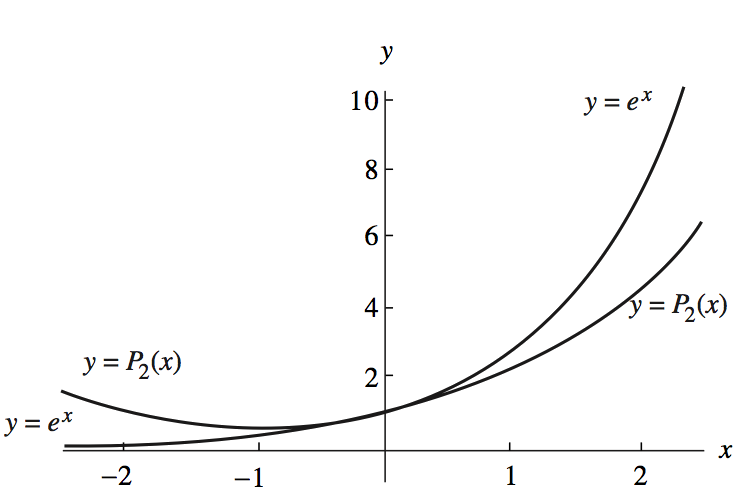
\includegraphics[width=70mm]{chap-3/fig_4-4.png}
\end{center}
\end{figure}
}

\frame{
\begin{itemize}
\item In the theory of approximation, one seeks to find an accurate polynomial approximation to the analytic function $f(x)$ over $[a, b]$. 
\item This is one technique used in developing computer software. 
\item The accuracy of a Taylor polynomial is increased when we choose $N$ large. 
\item The accuracy of any given polynomial will generally decrease as the value of $x$ moves away from the center $x_0$. 
\item Hence we must choose $N$ large enough and restrict the maximum value of $|x - x_0|$ so that the error does not exceed a specified bound. 
\end{itemize}
}

\frame{
\begin{itemize}
\item If we choose the interval width to be $2R$ and $x_0$ in the center (i.e., $|x-x_0| < R$), the absolute value of the error satisfies the relation 
\begin{equation*}
|error| = |E_N(x)| \le \frac{MR^{N+1}}{(N+1)!}
\end{equation*}
where $M \ge  \max{| f^{(N+1)}(z)| : x_0 - R \le z \le x_0 + R}$. 
\item If the derivatives are uniformly bounded, the error bound in (3.8) is proportional to $R^{N+1} / (N + 1)!$ and decreases for fixed $R$, when $N$ gets large or, for fixed $N$, when $R$ goes to 0. 
\end{itemize}
}

\frame{
Table 3.3 shows how the choices of these two parameters affect the accuracy of the approximation $e^x \approx P_N(X)$ over the interval $|x| \le R$. 
\begin{figure}
\begin{center}
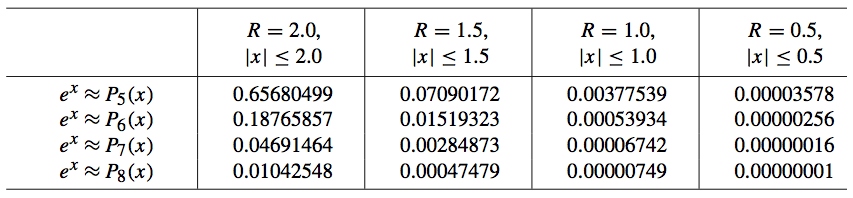
\includegraphics[width=100mm]{chap-3/tab_4-3.png}
\end{center}
\end{figure}
}

\frame{
\begin{itemize}
\item The error is smallest when $N$ is largest and $R$ smallest. 
\item Graphs for $P_2$, $P_3$, and $P_4$ are given in Figure 3.5. 
\end{itemize}
\begin{figure}
\begin{center}
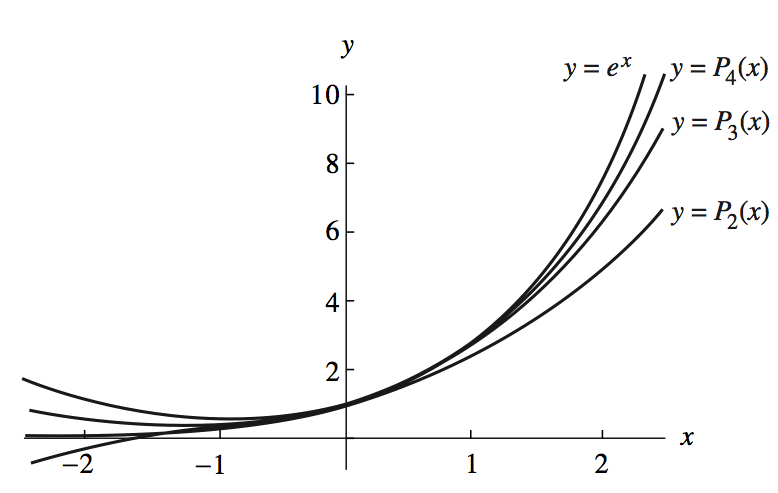
\includegraphics[width=70mm]{chap-3/fig_4-5.png}
\end{center}
\end{figure}
}

\frame{
\frametitle{Example 3.2.}
Establish the error bounds for the approximation $e^x \approx P_8(x)$ on each of the intervals $|x| \le 1.0$ and $|x| \le 0.5$.

If $|x| \le 1.0$, then letting $R = 1.0$ and $| f^{(9)}(c)| = |e^c| \le e^{1.0} = M$  implies that
\begin{equation*}
\left| error \right| = \left| E_8 (x) \right| \le \frac{e^{1.0}(1.0)^9}{9!} \approx 0.00000794
\end{equation*}
If $|x| \le 0.5$, then letting $R = 0.5$ and $| f^{(9)}(c)| = |e^c| \le e^{0.5} = M$ implies that
\begin{equation*}
\left| error \right| = \left| E_8 (x) \right| \le \frac{e^{0.5}(0.5)^9}{9!} \approx 0.00000001
\end{equation*}
}

\frame{
\frametitle{Example 3.3.}
If $f(x) = e^x$, show that $N = 9$ is the smallest integer, so that the $|error| = |E_N(x)| \le 0.0000005$
for $x$ in $[-1,1]$. 
\begin{itemize}
\item Hence $P_9(x)$ can be used to compute approximate values of $e^x$ that will be accurate in the sixth decimal place. 
\item We need to find the smallest integer $N$ so that 
\begin{equation*}
| error | = | E_N(x) | \le \frac{e^c (1)^{N+1}}{(N+1)!} < 0.0000005
\end{equation*}
\end{itemize}
}

\frame{
\begin{itemize}
\item In Example 3.2 we saw that $N = 8$ was too small, so we try $N = 9$ and discover that $|E_N(x)| \le  e^1(1)^{9+1} \/ (9 + 1)! \le 0.000000749$. 
\item This value is slightly larger than desired; hence we would be likely to choose $N = 10$. 
\item But we used $e^C \le e^1$ as a crude estimate in finding the error bound. 
\item Hence $0.000000749$ is a little larger than the actual error. 
\item Figure 3.6 shows a graph of $E_9(x) = e^x - P_9(x)$. 
\end{itemize}
}

\frame{
\begin{figure}
\begin{center}
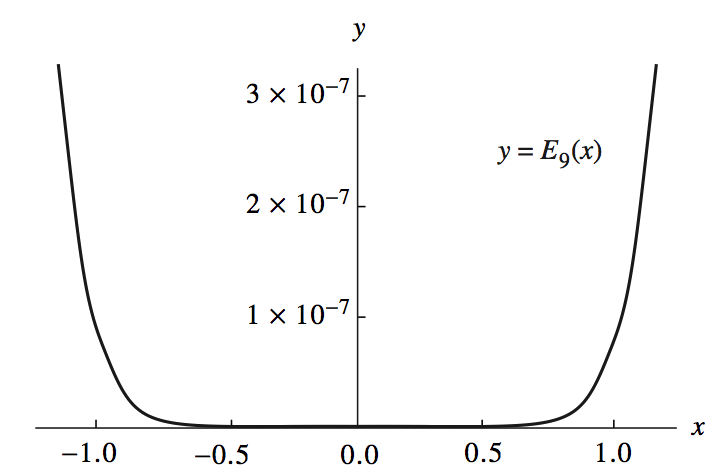
\includegraphics[width=70mm]{chap-3/fig_4-6.png}
\end{center}
\end{figure}
\begin{itemize}
\item Notice that the maximum vertical range is about $3 \times 10^{-7}$ and occurs at the right endpoint $(1, E_9(1))$. 
\item Indeed, the maximum error on the interval is $E_9(1) = 2.718281828 - 2.718281526 \approx 3.024 \times 10^{-7}$. 
\item Therefore, $N = 9$ is justified. 
\end{itemize}
}

\frame{
\frametitle{Methods for Evaluating a Polynomial}
There are several mathematically equivalent ways to evaluate a polynomial. 
Consider, for example, the function
\begin{equation*}
f(x) = (x-1)^8
\end{equation*}
The evaluation of f will require the use of an exponential function. 
Or the binomial formula can be used to expand $f(x)$ in powers of $x$:
\begin{equation*}
\begin{array}{l c l}
f(x) & = & \sum_{k=0}^8 x^{8-k} (-1)^k \\
& = & x^8 - 8 x^7 + 28x^6 - 56x^5 + 70x^4 - 56x^3 + 28x^2 - 8^x + 1
\end{array}
\end{equation*}
}

\frame{
\begin{itemize}
\item {\Large Horner's method}, which is also called {\Large nested multiplication}, can now be used to evaluate the polynomial in (3.10). 
\item When applied to formula (3.10), nested multiplication permits us to write 
\begin{equation*}
f (x) = (((((((x - 8)x + 28)x - 56)x + 70)x - 56)x + 28)x - 8)x + 1
\end{equation*}
\end{itemize}
\begin{block}{}
\begin{itemize}
\item To evaluate f(x) now requires seven multiplications and eight additions or subtractions. 
\item The necessity of using an exponential function to evaluate the polynomial has now been eliminated. 
\end{itemize}
\end{block}
}

\frame{
\begin{block}{Theorem 3.2 (Taylor Series).} 
Assume that $f (x)$ is analytic on an interval $(a, b)$ containing $x_0$. 
Suppose that the Taylor polynomials tend to a limit
\begin{equation*}
S(x) = \lim_{N \rightarrow \infty} P_N(x) = \lim_{N \rightarrow \infty} \sum_{k=0}^{N} \frac{f^{(k)} (x_0) }{k!} (x -x_0)^k
\end{equation*}
then $f (x)$ has the Taylor series expansion
\begin{equation*}
f(x) =  \sum_{k=0}^{N} \frac{f^{(k)} (x_0) }{k!} (x -x_0)^k
\end{equation*}
\end{block}
}

\frame{
Proof  of Theorem 3.2: \\
The limit condition is often stated by saying that the error term must go to zero as $N$ goes to infinity. 

Therefore, a necessary and sufficient condition for $f(x)$ to hold is that
\begin{equation*}
\lim_{N \rightarrow \infty} E_N(x) =  \lim_{N \rightarrow \infty} \frac{f^{(N+1)} (c) (x -x_0)^{N+1}}{(N+1)!} = 0
\end{equation*}
where $c$ depends on $N$ and $x$.
} 


